\documentclass[10pt,twocolumn]{article}

% ── Packages ──────────────────────────────────────────────────────────
\usepackage[utf8]{inputenc}
\usepackage[T1]{fontenc}
\usepackage{times}
\usepackage[margin=0.75in,top=0.7in,bottom=0.7in,columnsep=0.3in]{geometry}
\usepackage{titlesec}
\usepackage{enumitem}
\usepackage{hyperref}
\usepackage{booktabs}
\usepackage{tabularx}
\usepackage{microtype}
\usepackage{amsmath,amssymb}
\usepackage{caption}
\usepackage{url}
\usepackage{tikz}
\usetikzlibrary{arrows.meta,positioning,shapes.geometric,fit,calc}

% ── Hyperlinks ────────────────────────────────────────────────────────
\hypersetup{
  colorlinks=false,
  pdfborder={0 0 0},
  pdftitle={DeltaScribe Edge: Offline Longitudinal CXR Copilot},
  pdfauthor={Simon},
}

% ── Section formatting ────────────────────────────────────────────────
\titleformat{\section}{\normalsize\bfseries}{\thesection.}{0.5em}{}
\titleformat{\subsection}{\small\bfseries}{\thesubsection}{0.5em}{}
\titlespacing*{\section}{0pt}{0.8em}{0.25em}
\titlespacing*{\subsection}{0pt}{0.5em}{0.15em}

% ── Compact lists ─────────────────────────────────────────────────────
\setlist[itemize]{leftmargin=1.2em,itemsep=1pt,parsep=0pt,topsep=2pt}
\setlist[enumerate]{leftmargin=1.4em,itemsep=1pt,parsep=0pt,topsep=2pt}

% ── Paragraph spacing ────────────────────────────────────────────────
\setlength{\parskip}{2.5pt plus 1pt}
\setlength{\parindent}{1em}

% ══════════════════════════════════════════════════════════════════════
\begin{document}

% ── Title ─────────────────────────────────────────────────────────────
\twocolumn[{%
\centering
{\Large\bfseries DeltaScribe Edge: Offline Longitudinal Chest X-Ray Copilot\\[2pt]
with Verifiable Evidence and FHIR Export\par}
\vspace{6pt}
{\normalsize The MedGemma Impact Challenge --- Kaggle 2026\par}
\vspace{10pt}
\rule{0.4\textwidth}{0.4pt}
\vspace{8pt}
}]
\thispagestyle{empty}

% ══════════════════════════════════════════════════════════════════════
\section{Project Name}

DeltaScribe Edge --- Offline longitudinal chest X-ray copilot with verifiable evidence and FHIR export.

% ══════════════════════════════════════════════════════════════════════
\section{Your Team}

\textbf{Simon} --- Architecture, implementation, and evaluation (independent, end-to-end development).

% ══════════════════════════════════════════════════════════════════════
\section{Problem Statement}

\subsection{Problem Domain}

Follow-up respiratory imaging is among the most common and time-critical workflows in clinical care (pneumonia follow-up, pulmonary edema monitoring, post-treatment assessment).
The core challenge is not interpreting a single image but answering: \emph{what changed since the prior study, and how should that change be documented consistently?}

Clinicians must locate the relevant prior, compare findings across studies, draft standardised interval-change language, and communicate uncertainty.
This process is structured and repetitive yet remains largely manual.
Many clinical environments cannot rely on large closed cloud models due to privacy constraints, limited connectivity, latency, and governance requirements.
Open-weight healthcare models enable local deployment with auditable behaviour, making AI-assisted longitudinal documentation feasible.

Today, the dominant workflow involves the radiologist opening both studies side-by-side, mentally cataloguing findings, and free-text dictating a report.
Variability across reporters is well-documented: identical imaging pairs can yield materially different interval-change assessments depending on time pressure, template availability, and individual reporting style.
A tool that produces a structured, evidence-linked first draft---subject to clinician review---can reduce this variability while preserving clinical judgment.

\subsection{Impact Potential}

An effective solution improves:
(1)~documentation efficiency via faster time-to-first-draft;
(2)~consistency through standardised delta language;
(3)~continuity of care for rotating staff; and
(4)~trustworthiness via explicit evidence mapping and uncertainty gating.

\smallskip
\noindent\textbf{Illustrative estimate.}
If a site drafts 30 follow-up CXR reports per day and saves 2~minutes per report, that yields ${\sim}$60~min/day (${\sim}$5~hours/week) of clinician time returned to direct care.
With an average time-to-first-draft of ${\sim}$135\,s on commodity hardware (Apple~M3 Air, CPU-only Docker), a 2-minute saving per report is achievable on GPU-equipped workstations.

% ══════════════════════════════════════════════════════════════════════
\section{Overall Solution}

DeltaScribe Edge is an offline-first demonstration application for longitudinal CXR follow-ups.
It accepts:

\begin{itemize}
  \item Current CXR/DICOM + Prior CXR/DICOM (required; native DICOM detection with VOI LUT windowing).
  \item Optional: dictation audio (brief clinician note).
  \item Optional: FHIR-formatted patient context (conditions, medications, prior report snippet).
\end{itemize}

\noindent It produces four outputs:

\begin{enumerate}
  \item \textbf{Delta Summary} --- concise interval-change bullets.
  \item \textbf{Draft Report} --- radiology-style Findings / Impression template.
  \item \textbf{Evidence Ledger} --- every claim linked to evidence sources and an uncertainty level.
  \item \textbf{FHIR R4 Export} --- a conformant Bundle containing \texttt{DiagnosticReport} and \texttt{Observation} resources with SNOMED~CT coding, generated by deterministic mapping from the structured output (the model does not write FHIR directly).
\end{enumerate}

\subsection{Why HAI-DEF / MedGemma}

MedGemma is purpose-built for medical multimodal reasoning, including CXR interpretation.
Open-weight healthcare models enable full control over weights and infrastructure, supporting offline, privacy-preserving deployment where care is delivered.

\smallskip
\noindent\textbf{HAI-DEF models used:}

\begin{itemize}
  \item \textbf{MedGemma 4B-IT} (text): narrative generation for longitudinal CXR reports and structured JSON output. Default: GGUF Q4\_K\_M (${\sim}$2.3\,GB) via \texttt{llama-cpp-python} for CPU/edge; multimodal transformers pathway available for GPU. In the CPU/edge GGUF configuration, MedGemma is text-only; image understanding is performed by MedSigLIP and BiomedCLIP.
  \item \textbf{MedASR} (optional): offline medical dictation (fallback chain: MedASR $\rightarrow$ Whisper).
  \item \textbf{MedSigLIP}: zero-shot pathology classification (finding detection) and cross-modal retrieval.
  \item \textbf{CXR Foundation}: precomputed atlas embeddings for similar-case retrieval.
\end{itemize}

% ══════════════════════════════════════════════════════════════════════
\section{Technical Details}

\subsection{Architecture}

A reproducible containerised stack:
\textbf{Frontend:} Next.js~16 + shadcn/ui (local web UI).
\textbf{Backend:} Python FastAPI orchestrator with WebSocket real-time status push.
\textbf{Runtime:} local model weights mounted into the container; no network access required.
\textbf{Assets:} 7~curated demo patient pairs, reference atlas, FHIR export templates.
All inference runs locally; no patient data needs to leave the device.

% ── Architecture Diagram ─────────────────────────────────────────────
\begin{figure}[h]
\centering
\resizebox{\columnwidth}{!}{%
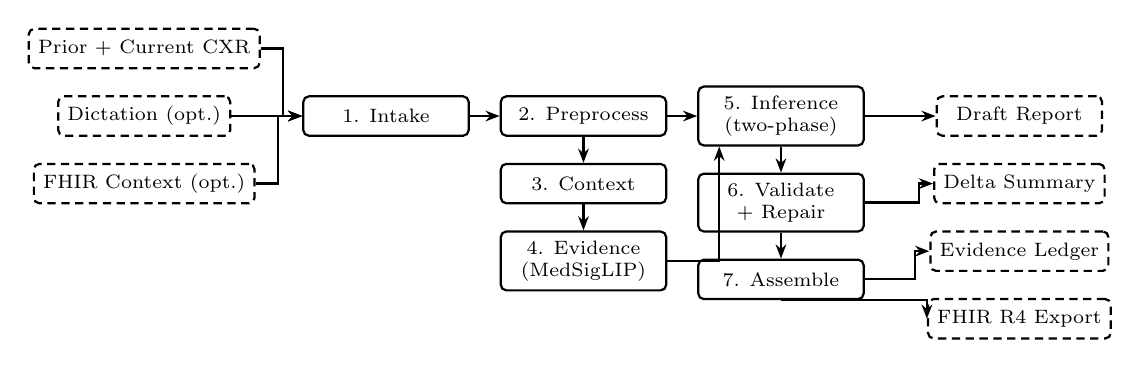
\begin{tikzpicture}[
    node distance=0.33cm and 0.38cm,
    every node/.style={font=\scriptsize},
    box/.style={draw, rounded corners=2pt, minimum height=0.5cm,
                minimum width=2.1cm, align=center, thick},
    io/.style={box, densely dashed},
    arrow/.style={-{Stealth[length=1.8mm]}, thick},
  ]
  \node[io] (cxr) {Prior + Current CXR};
  \node[io, below=of cxr] (audio) {Dictation (opt.)};
  \node[io, below=of audio] (fhir_in) {FHIR Context (opt.)};
  \node[box, right=0.9cm of audio] (val) {1. Intake};
  \node[box, right=of val] (pre) {2. Preprocess};
  \node[box, below=of pre] (ctx) {3. Context};
  \node[box, below=of ctx] (rag) {4. Evidence\\(MedSigLIP)};
  \node[box, right=of pre] (inf) {5. Inference\\(two-phase)};
  \node[box, below=of inf] (schema) {6. Validate\\+ Repair};
  \node[box, below=of schema] (ledger) {7. Assemble};
  \node[io, right=0.9cm of inf] (report) {Draft Report};
  \node[io, below=of report] (delta) {Delta Summary};
  \node[io, below=of delta] (ev) {Evidence Ledger};
  \node[io, below=of ev] (fhir_out) {FHIR R4 Export};
  \draw[arrow] (cxr.east) -- ++(0.28,0) |- (val.west);
  \draw[arrow] (audio.east) -- (val.west);
  \draw[arrow] (fhir_in.east) -- ++(0.28,0) |- (val.west);
  \draw[arrow] (val) -- (pre);
  \draw[arrow] (pre) -- (inf);
  \draw[arrow] (pre.south) -- (ctx.north);
  \draw[arrow] (ctx.south) -- (rag.north);
  \draw[arrow] (rag.east) -| ($(inf.south west)+(0.28,0)$);
  \draw[arrow] (inf) -- (schema);
  \draw[arrow] (schema) -- (ledger);
  \draw[arrow] (inf.east) -- (report.west);
  \draw[arrow] (schema.east) -| ($(delta.west)-(0.18,0)$) -- (delta.west);
  \draw[arrow] (ledger.east) -| ($(ev.west)-(0.18,0)$) -- (ev.west);
  \draw[arrow] (ledger.south) -| (fhir_out.west);
\end{tikzpicture}%
}
\caption{Agentic pipeline. Dashed boxes are inputs/outputs; solid boxes are deterministic tool steps. Each step emits a WebSocket event to the real-time UI timeline.}
\label{fig:pipeline}
\end{figure}

\subsection{Agentic Workflow (7-Step State Machine)}

DeltaScribe Edge decomposes the clinical workflow into a \emph{deterministic state machine} with 7~explicit tool steps (Figure~\ref{fig:pipeline}), each emitting a WebSocket event to a real-time UI timeline:

\begin{enumerate}
  \item \textbf{Intake} --- verify prior/current imaging present (native DICOM detection + VOI LUT windowing); check optional inputs.
  \item \textbf{Preprocess} --- normalise images to consistent internal format.
  \item \textbf{Retrieve Context} (optional) --- parse FHIR bundle fields; transcribe dictation via MedASR/Whisper.
  \item \textbf{Retrieve Evidence} --- MedSigLIP zero-shot classification (8 pathology classes across 13 candidate labels) to detect candidate findings; BiomedCLIP (Microsoft, via \texttt{open\_clip}) image RAG retrieves top-$K$ similar cases from the CXR Foundation atlas.
  \item \textbf{Inference (two-phase)} ---
    \emph{Phase~1:} MedSigLIP provides structured finding detection (labels + confidence).
    \emph{Phase~2:} MedGemma 4B-IT receives the detected findings, retrieval evidence, and patient context as a structured prompt, and generates the narrative report and structured JSON.
    Classification agreement between MedSigLIP and MedGemma is tracked per case.
  \item \textbf{Validate + Repair} --- enforce strict JSON schema; auto-repair fills missing \texttt{evidence\_refs} with \texttt{["current\_image"]} and downgrades uncertainty to \textit{high} if needed.
  \item \textbf{Assemble} --- build Evidence Ledger with uncertainty gating (supporting/conflicting evidence $\rightarrow$ accept/flag/reject), draft report, and FHIR R4 Bundle (\texttt{DiagnosticReport} + \texttt{Observations} with SNOMED~CT codes).
\end{enumerate}

The two-phase design separates \emph{what} is found (MedSigLIP, inspectable) from \emph{how} it is narrated (MedGemma, auditable), enabling cross-validation and matching the Agentic Workflow Prize intent.

\subsection{Evidence Ledger}

Each finding is a \emph{claim object}: (i)~claim text, (ii)~evidence pointers (current/prior image, similar cases, dictation excerpts), (iii)~uncertainty level $\in \{\textit{low},\, \textit{medium},\, \textit{high}\}$, and (iv)~clinician-readable rationale on the Finding, linked via audit trail.

The schema requires every finding to link $\geq$1 evidence source (\texttt{evidence\_refs: min\_length=1}); findings without evidence cannot pass validation.
If the repair pass encounters an empty list, it auto-fills \texttt{["current\_image"]} and sets uncertainty to \textit{high}, signalling that the finding lacks model-provided evidence.

% ── Evidence Ledger Example ──────────────────────────────────────────
\begin{table}[h]
\centering
\small
\caption{Example Evidence Ledger entry.}
\label{tab:ledger_example}
\begin{tabularx}{\columnwidth}{@{}lX@{}}
\toprule
\textbf{Field} & \textbf{Value} \\
\midrule
Claim       & Pleural effusion improved vs.\ prior. \\
Evidence    & Current CXR, Prior CXR, 5 similar cases (BiomedCLIP), 13 zero-shot labels (MedSigLIP). \\
Uncertainty & \textit{low} \\
Rationale   & Effusion extent decreased; MedSigLIP and MedGemma agree on effusion label with improved delta. \\
\bottomrule
\end{tabularx}
\end{table}

\subsection{Retrieval}

\textbf{Image RAG.}
BiomedCLIP (Microsoft, non-HAI-DEF) encodes the query CXR; top-$K$ similar cases retrieved from CXR Foundation atlas via cosine similarity (5 per demo case, displayed with scores).

\textbf{Zero-shot classification.}
MedSigLIP classifies 13 candidate labels with confidence scores for Phase~1 finding detection.

\noindent Guideline retrieval is architecturally supported but currently disabled (no licensed data bundled).
All retrieval artifacts are visible in the UI for clinician inspection.

\subsection{Key Design Decisions}

\begin{enumerate}
  \item \textbf{Two-phase inference, not monolithic generation.}
  MedSigLIP detects findings (Phase~1); MedGemma narrates (Phase~2).
  Classification agreement is tracked; disagreements can be flagged.

  \item \textbf{Structured intermediate representation.}
  JSON schema per finding: \texttt{label} (8-class), \texttt{delta} (improved/stable/worsened/uncertain), \texttt{rationale}, \texttt{evidence\_refs}, optional \texttt{bounding\_box}, \texttt{uncertainty}.
  The draft report is rendered \emph{from} this structure, ensuring consistency.

  \item \textbf{Retrieval as context and transparency.}
  Similar cases and zero-shot classifications are injected into the MedGemma prompt and surfaced in the UI for independent verification.

  \item \textbf{FHIR R4 + SNOMED~CT as a first-class output.}
  Deterministic mapping with 8 SNOMED~CT code mappings at every run.
\end{enumerate}

\subsection{Evaluation}

\begin{table}[h]
\centering
\small
\caption{Results over 7 demo pairs (Apple M3 Air, CPU-only Docker).}
\label{tab:eval}
\begin{tabularx}{\columnwidth}{@{}lXr@{}}
\toprule
\textbf{Category} & \textbf{Metric} & \textbf{Result} \\
\midrule
Reliability & Schema validity (no repair needed) & 7/7 \\
            & FHIR R4 export integrity    & Pass \\
Feasibility & Latency (avg / range)       & 135\,s / 30--231\,s \\
Consistency & Delta agreement (NIH-derived proxy labels) & 71\% (5/7) \\
            & MedSigLIP--MedGemma agreement & tracked \\
Trust       & Evidence coverage            & 100\% \\
            & Evidence per case            & 5 sim.\ + 13 zs \\
            & Disclaimer present           & 100\% \\
Interop.    & SNOMED~CT codes mapped       & 8/8 \\
\bottomrule
\end{tabularx}
\end{table}

\noindent\textbf{Protocol.}
7~demo pairs run end-to-end in Docker on Apple~M3 Air (24\,GB RAM, CPU-only, GGUF Q4\_K\_M).
cxr\_001 is slowest (231\,s) due to cold loading of 3~models (GGUF + BiomedCLIP + MedSigLIP, ${\sim}$60\,s); cxr\_006/007 run in ${\sim}$30\,s with warm models.
Delta label agreement: 71\% (5/7) against NIH-derived proxy labels (per-image NIH labels $\rightarrow$ logical delta derivation for prior/current pairs; weak supervision, not expert annotation).
Evidence coverage: all asserted findings include $\geq$1 valid evidence pointer.
All evaluation code and reproduction commands are in \texttt{EVALUATION.md}.

\subsection{Responsible Use and Limitations}

DeltaScribe Edge is \emph{not} a diagnostic device.
Outputs are drafts intended for review by qualified clinicians.
The system requires both prior and current imaging; analysis cannot proceed without paired studies.
Retrieval is used for transparency---not for ``diagnosis by similarity.''
All inference runs locally; no PHI needs to leave the device.

Known limitations: bounded by MedGemma's training distribution; small demo atlas; guideline retrieval disabled (no licensed data); single-modality (CXR) only; prototype UI.

\subsection{Future Work}

Fine-tuning MedGemma on annotated longitudinal pairs to improve beyond 71\% delta agreement; scaling the atlas and licensing guideline content for text RAG; CT and multi-modality extension; clinical pilot with IRB approval.

\subsection{What the Video Demonstrates}

\begin{itemize}
  \item Offline proof (no network during inference).
  \item DICOM loading with VOI LUT windowing.
  \item Real-time WebSocket agent timeline.
  \item Two-phase inference: MedSigLIP detection $\rightarrow$ MedGemma narrative.
  \item Evidence Ledger inspection (claim $\rightarrow$ source tracing).
  \item FHIR R4 export with SNOMED~CT codes.
\end{itemize}

% ══════════════════════════════════════════════════════════════════════
\section{Links}
\label{sec:links}

\noindent\textbf{Track selection:} Main Track + Agentic Workflow Prize.

\smallskip
\noindent\textbf{Required:}
\begin{itemize}
  \item Video demo ($\leq$3\,min): uploaded directly to Kaggle submission.
  \item Public code repository: \url{https://github.com/simonrueba/deltascribe-edge}
\end{itemize}

% ══════════════════════════════════════════════════════════════════════
\bibliographystyle{plain}
\begin{thebibliography}{1}
\small
\bibitem{medgemma2026}
F.~Mahvar et al.
\newblock The {MedGemma} Impact Challenge.
\newblock \url{https://kaggle.com/competitions/med-gemma-impact-challenge}, 2026.
\end{thebibliography}

\end{document}
